\documentclass{article}

\usepackage{titlesec}
\usepackage[margin=1 in]{geometry}
\usepackage{graphicx}
\usepackage{subfig}

\graphicspath{ {./Figures/} }
\setlength{\columnsep}{1cm}
\title{Theoretical Universal Scaling in the Dynamics of Yukawa One-Component Plasmas}
\author{M. Andrew Sampson}
\newcommand{\sgn}{\mathop{\mathrm{sgn}}}
\begin{document}
\maketitle 
\renewcommand\abstractname{}
\begin{abstract}
This paper analyzes the effects on the motion, velocity, angular momentum, and energy of universal scaling on the Yukawa One-Component Plasma (OCP) model using computational methods. We prove that the nonlinear motion of the OCP model becomes densely chaotic at high wave vector values and is extremely sensitive to scaling at even low wave vector values. We find that the velocity of the system is scaled inversely by the scaling parameter, that the angular momentum of the system is directly scaled by the scaling parameter, and that the energy of the system is scaled inversely by the square of the scaling parameter. In a lab environment, the results of this research could be used to artificially control the flow of ultra-cold plasma by varying the volume of the plasma's container, the temperature of the plasma, or the pressure of the plasma.
\end{abstract}

\section{Introduction}
					
In studying strongly coupled Coulomb systems, the Yukawa One-Component Plasma (OCP) model provides a simple model for describing certain properties useful in ultra-cold ionic systems- such as those seen in the cores of dwarf stars and Jovian planets, ions in ultra-cold
neutral plasmas, and highly-charged dusty plasmas\cite{ocp1}. In the OCP model, a system of similarly charged point particles interact classically and exclusively through the Coulomb potential, making it especially useful for studying low-energy systems.

Additionally, the OCP model varies by a single parameter,
\begin{equation}
\Gamma = \frac{E_{C}}{kT_{e}}
\end{equation}
referred to as the Coulomb coupling parameter, where $E_{C}$ is the Coulomb energy, k is Boltzmann's constant, and $T_{e}$ is the electron temperature. Eq. (1) can also be written as
\begin{equation}
\Gamma = \frac{q_{e}^2}{4\pi \epsilon_{0} \vec{r}kT_{e}}
\end{equation}
where $\vec{r}$ is the  Wigner-Seitz radius\cite{ocp2}. This parameter dictates how strongly coupled the plasma is, and is essential in understanding its dynamics.

Now consider the motion of n charged particles in an ultra-cold, strongly coupled plasma described by the position vector
$\vec{r}$ under the scaling transformation, with arbitrary scaling parameter a:
\begin{equation}
\vec{r} \to r'= a^2 \vec{r}
\end{equation}

and
\begin{equation}
t \to t'= a^3 t
\end{equation}

The equation of motion is invariant, meaning that if ~r(t) is known to be a solution, then
the scaled transformation of that is also a solution. So, if our new position vector $\vec{r}$ is defined to be the Wigner-Seitz radius, then scaling it under eq. (3) should also change other properties of the OCP system.

In this paper, we will explore how this universal scaling affects the motion, velocity, angular momentum, and energy of the system and, in the process, develop a deeper understanding of scaling in chaotic systems and applications of nonlinear dynamics in plasma physics.

\section{Motion Under Universal Scaling}
\subsection{The Zaslavskii Map}
Due to the nature of the OCP model, the motion of an electron in the system can be described using the nonlinear Zaslavskii Map constructed by
\begin{equation}
x_{n} = x_{n-1} + y_{n} \pmod 1
\end{equation}
\begin{equation}
y_{n} = c y_{n-1} + k \sin{(2 \pi x_{n-1})}
\end{equation}
where $c < 1$ and k is the wave vector, expressed as 
\begin{equation}
k = \frac{2 \pi}{\lambda}
\end{equation}
with $\lambda$ representing the wavelengths of the electromagnetic waves given off from the motion of surrounding particles in the system\cite{ocp3}. 

Perhaps the most interesting and useful thing about this mapping is the group of nonlinear systems it belongs to. What's so interesting about that? Well, the Zaslavskii Map happens to belong to a group of attractors called \textit{strange attractors}. That is to say that this Zaslavskii Map is a recursive aperiodic mapping where the flow is evolving around a subset of points, called attractors. And it is this behavior that provides important insight on the behavior we can expect from mapping the motion of an electron in our OCP system. The first, and most important thing we know about the system comes from its definition; it is an aperiodic attractor. This tells us that (1) the motion will be chaotic and (2) there is a subset of points that the electron will naturally gravitate towards, providing a more useful way to talk about the attractor's motion. Second, we know that the attractor has a fractal structure\cite{ocp4}, and therefore follows a period bifunction pattern\cite{ocp5}.

Returning back to the wave vector, we first need to have it in terms of $\vec{r}$ before we can do anything useful with our scaling transformation. Rewriting eq. (7), we get:
$$k = \frac{2 \pi E}{hc}$$
and substituting $E = \frac{k_{e}q_{1}q_{2}}{r}$ and summing for all charges in the system gives:
\begin{equation}
k = \frac{-2 \pi k_{e} e^2}{hc} \sum_{i=1}^n \frac{\sgn(q_{i})}{\vec{r}_{i}}
\end{equation}
where $k_{e}$ is Boltzmann's constant and e is the charge of an electron. And since $k \propto \frac{1}{\vec{r}}$, under the scaling in eq. (3) we get our first result:
\begin{equation}
k \to k' = \frac{k}{a^2}
\end{equation}

While, at first, this result may seem trivial and only arising from the scaling transformation, it will soon prove useful when considering its effect on the chaotic motion of our electron, as displayed in Fig. 2(a) and 1(b) and later in Fig. 1 when we discuss period bifurcation.

\subsection{Cyclic Nature and Chaos at $k >> 0$}
Now that we've found the scaled value of k, we have everything we need to fully examine the motion of an electron in our system. But what happens as k is varied? We will see that as k increases, the number of attractors in the system will grow as it undergoes period doubling; that is, the number of attractors in the system will double after some increase in k since the last doubling as seen in Fig. 1. To understand Fig. 1, observe first that, (1) since the system is exhibiting period doubling behavior, the interval of k since the last doubling as k becomes large must shrink by a factor of $\delta = 4.669...$\cite{ocp5} and, more interestingly, (2) as k becomes larger, the doubling "resets", that is, the number of attractors in the system returns to 2, over an interval, $\gamma$ that approaches some value as k tends to infinity. Thus, $\gamma$ is defined as:
$$\gamma = x_{b_{n}} - x_{b_{n-1}}$$
where $x_{b_{n}}$ is the nth "reset" and $\gamma$ (quickly) approaches the constant value of 1.1.
What this tells us is that, at very large values of k, the function space of the Zaslavskii Map as it varies by k becomes dense with attractors, making the system much more sensitive to scaling. For our electron, this means for values of $k >> 0$ with few attractors, even a scaling parameter just over or under 1 is likely to cause it to exhibit chaotic motion. Additionally, the period doubling of the Zaslavskii Map turns quite chaotic at low values of k, causing the interval between successive doublings to be quite small very quickly. Consequentially, this small interval between doublings also means that it only takes relatively small values of a to turn the motion of an electron chaotic, as seen in Fig. 2(a) and (b).

\begin{figure}[t!]
\label{Fig. 2}
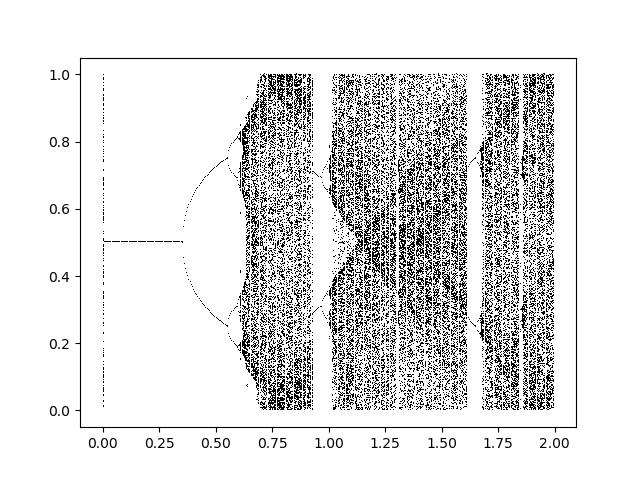
\includegraphics[scale=1]{Logistic_Graph}
\caption{Period doubling sequence of the Zaslavskii Map}
\end{figure}

\begin{figure}[h!]
\label{Fig. 2}
\subfloat[original mapping]{\label{sublable1}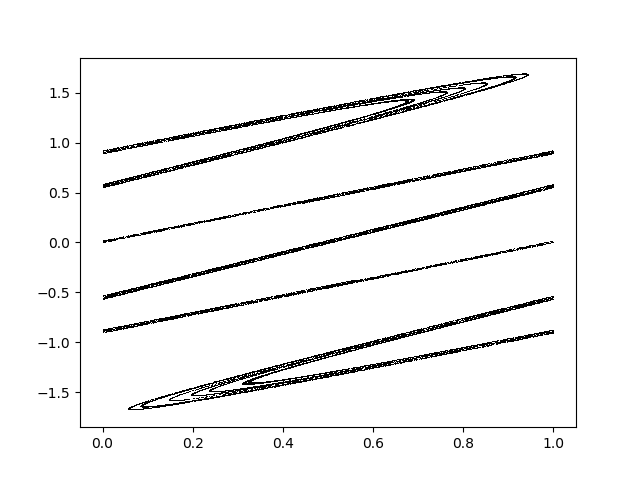
\includegraphics[scale=0.8]{l=0,1;k=1,57,50000pts;x=0,1;y=0,1}} \\
    \subfloat[mapping with $a = 1.0158$. Points were enlarged to improve visibility.]{\label{sublable2}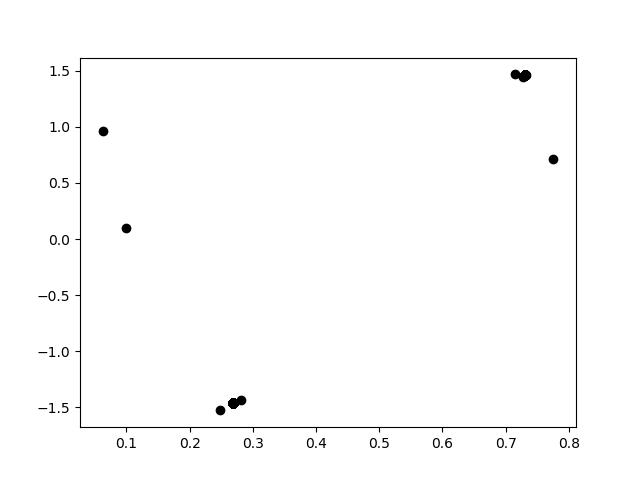
\includegraphics[scale=0.8]{l=0,1;k=1,62;20000pts;x=0,1;y=0,1}}
    \caption{$\lambda = 0.1$, $k = 1.57$, and initial point of (0.1,0.1). (a) shows an extremely chaotic pattern while (b) is mainly concentrated around 2 points (its attractors)}
\end{figure}
\newpage

\section{Scaling of Other Properties}
Now that we understand the motion of one electron in the scaled OCP system, let's now consider how the dynamics of the entire system change under our scaling transformation: namely, its velocity, angular momentum, and energy. But how might we possibly take into account the motion of all of the particles in the system? The key realization is that the state a system of particles can be found by considering the center of mass for all of the particles in the system: represented by
\begin{equation}
\vec{r}_{cm} = \frac{1}{M_{tot}} \sum_{i=1}^n m_i \vec{r}_i
\end{equation}

where $\vec{r}_{cm}$ is the position vector of the center of mass of the system and $M_{tot}$ is the total mass of the system.

Using the center of mass equation (10), we have
\begin{equation}
\vec{v} = \frac{d \vec{r}_{cm}}{dt}
\end{equation}


\begin{equation}
\vec{L} = M_{tot} \vec{v} \vec{r}_{cm}
\end{equation}
and (using the electron Hamiltonian)

\begin{equation}
H =\frac{e^2}{8 \pi \epsilon_0} \sum_{i=1}^n \frac{\sgn(q_{i})}{ \vec{r}_i}
\end{equation}
Under the scaling in eq. (3) and eq. (4) we have that
\begin{equation}
\vec{r}_{cm} \to r'_{cm} = a^2 \vec{r}_{cm}
\end{equation}
so the velocity scales to
\begin{equation}
\vec{v} \to v' = \frac{\vec{v}}{a}
\end{equation}
the angular momentum scales as
\begin{equation}
\vec{L} \to L' = a\vec{L}
\end{equation}

and the Hamiltonian will scale as
\begin{equation}
H \to H' = \frac{H}{a^2}
\end{equation}

\section{Summary and Discussion}
In this paper, we have reviewed some properties of the Yukawa One-Component Plasma model and how it behaves under a universal scaling transformation using nonlinear dynamics and methods from computational analysis. We have shown that the wave vector is scaled by the square of the inverse of our transformation scalar, a, and demonstrated that this leads to a very sensitive change in the chaotic motion of an electron in the system. We have shown that, due to the rapid doubling of the Zaslavskii Map and its tendency to "reset" its doubling, that the motion of an electron in the system is very sensitive to scaling with even a small k. And we derived the transformations of the velocity, angular momentum, and energy of the whole system.

The findings of this study are consistent with those of Rice University (2015)\cite{ocp1}, where they experimentally tested the effects of scaling in the Quench Dynamics of a similar OCP. Taken together, these findings suggest that the chaotic motion found in the extreme examples of OCP's, such as those with very weak or very strong coupling, can be understood through simple, nonlinear systems like the Zaslavskii Map. Further research must be done on understanding the "resetting" of the Zaslavskii Map as the tendency  of the interval between the "resets" towards 1.1 is currently unexplained. Regarding the universal scaling transformation, broadening the extent of study in applying transformations to unpredictable models may lead to a deeper understanding of the fundamental processes at work in them and broader connections to other, perhaps more studied, nonlinear systems.

In a lab environment, the results of this research could be used to artificially control the flow of ultra-cold plasma by varying the volume of the plasma's container, the temperature of the plasma (very slightly so it still mainly interacts through the Coulomb-Kepler interaction), or the pressure of the plasma. By doing this, researchers could funnel the plasma into 1, 2, or however many points they want or create chaotic motion! Further research is needed to verify and perform this technique.
\begin{thebibliography}{9}
\bibitem{ocp1} 
K. Langin, T \& Strickler, T \& Maksimovic, N \& Mcquillen, P \& Pohl, Thomas \& Vrinceanu, Daniel \& C. Killian, T. (2015). 
\textit{Demonstrating Universal Scaling in Quench Dynamics of a Yukawa One-Component Plasma.}

\bibitem{ocp2}
M. Baus and J.P. Hansen, \textit{Statistical Mechanics of Simple Coulomb Systems}, Phys. Rep. 50, 1 (1980).

\bibitem{ocp3}
T.H. stix , \textit{Stochasticit y and Superadiabaticit y in Radiofrequency Plasma
Heating} , Princeton Plasma Physics Laboratory Report PPPL-1539 (1979) 

\bibitem{ocp4}
Boeing, G. 2016. \textit{Visual Analysis of Nonlinear Dynamical Systems: Chaos, Fractals, Self-Similarity and the Limits of Prediction.} Systems, 4 (4), 37.

\bibitem{ocp5}
Feigenbaum, Mitchell. (1983). \textit{Universal Behavior in Nonlinear Systems}. Physica D: Nonlinear Phenomena. 7. 16-39. 10.1016/0167-2789(83)90112-4. 

\end{thebibliography}
\end{document}